\section{Measuring Phrase Anticipation}
\label{sec:method}

\begin{figure*}[t]
\centering
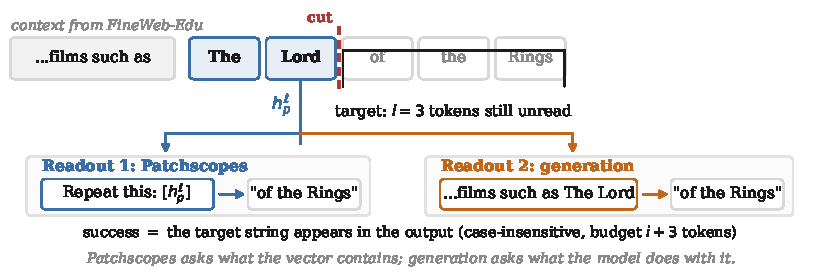
\includegraphics[width=\textwidth]{figures/protocol}
\caption{The protocol. We interrupt the model inside a known phrase, leaving $i$
tokens unread, and ask whether those tokens are recoverable from that point by
two different means: injecting the hidden state into an unrelated prompt
(Patchscopes), or letting the model continue from the prefix it has actually
seen (generation). Both are scored identically. In both, only the first token is
produced from the state shown; decoding then continues autoregressively, so a
multi-token recovery does not imply that every token was separately encoded in
$h^{\ell}_p$.}
\label{fig:protocol}
\end{figure*}

Figure~\ref{fig:protocol} summarises the protocol.

\subsection{Lookahead distance}

Let a phrase tokenize as $t_1 \ldots t_n$. We interrupt the model at position
$p$ and define the \emph{lookahead distance} $i = n - p$ as the number of phrase
tokens that remain unread. The target is the decoded string of those $i$ tokens.
A single phrase therefore yields several trials, one per position, and $i$ is
the difficulty axis throughout: larger $i$ means the model must account for more
unseen material.

Every phrase is processed with its full left context (a BOS token, then,
where applicable, the natural text preceding the phrase), so the state at
position $p$ is the state the model would actually have at that point. We analyse
$i \geq 2$ throughout; $i=1$ reduces to ordinary next-token prediction and is
not of interest here.

\subsection{Two readouts}
\label{sec:readouts}

We ask whether the remaining tokens are recoverable from the model at position
$p$ in two ways. Both take the same input and differ only in what is done with
it.

\paragraph{Patchscopes readout.}
Following \citet{ghandeharioun-etal-2024-patchscopes}, and ultimately the causal
intervention of \citet{pal-etal-2023-future}, we take the hidden state
$h^{\ell}_p$ at layer $\ell$ and position $p$, and substitute it for the token
embedding of \texttt{X} in the prompt \texttt{"Repeat this: X"}. We then decode
greedily for $i+3$ tokens. The readout succeeds at layer $\ell$ if the target
string occurs in the output, case-insensitively. Unless stated otherwise we
report the union over layers: the readout succeeds if \emph{any} probed layer
succeeds. This is a deliberately generous criterion, and \S\ref{sec:disagreement}
shows that how many layers enter the union materially changes the result.

\paragraph{Generation readout.}
We take the same prefix, context plus the first $p$ phrase tokens, and let
the model generate greedily for $i+3$ tokens, with no intervention of any kind.
The readout succeeds under the same string-containment criterion.

Neither readout is ground truth for the other, and they are not two decoders of
the same object. Patchscopes intervenes on a single hidden state and asks what
that vector can be made to express; generation runs the full model on the
matched prefix and asks what it does. The comparison is therefore between
representational extractability and behaviour, and we treat them as two
instruments rather than two views (\S\ref{sec:disagreement}).

One consequence is worth stating before any results. Both readouts decode
autoregressively, so a recovered target of several tokens does not show that
each of those tokens is separately encoded in the cut-position state: after the
first generated token, the rest may follow from what has already been emitted.
What a success shows is that the state carries enough information to elicit the
continuation under that readout. We use \emph{recognition} and
\emph{anticipation} in that operational sense throughout: a phrase is
recognized at distance $i$ when a named readout recovers its remaining $i$
tokens under the matching criterion below.

\subsection{Success criterion}
\label{sec:criterion}

A trial succeeds if the target string appears as a case-insensitive substring of
the generated continuation. The budget of $i+3$ tokens allows the model to
overshoot slightly (a trailing clause after the phrase does not cost it the
trial) while remaining tight enough that a success reflects the phrase
rather than a long ramble that happens to contain it.\footnote{An earlier
version of this work used a fixed five-token budget, which mechanically forced
zero successes at $i \geq 6$. The reported $i \geq 6$ rates here are the
corrected ones.}

The criterion is lenient in one direction and strict in the other. Lenient,
because it accepts any output containing the target without asking whether the
model produced it for the right reason; strict, because it demands the exact
wording: \textit{he who laughs last laughs \underline{best}} scores as a
failure against \textit{laughs loudest}, though it is the more common form.
\S\ref{sec:falsepos} quantifies how often that strictness misclassifies a
correct completion.
